\subsection{Our Contributions}

We make four contributions to the area of
privacy-preserving smart contracts:

\begin{enumerate}[label={\alph*)}]
  \item We \textbf{model} privacy-preserving smart contracts.
  \item We \textbf{realize a large class} of such contracts.
  \item We \textbf{enable concurrent interactions} with smart contracts,
    without compromizing on privacy.
  \item We demonstrate a general methodology to \textbf{efficiently and
      composably build} smart contract systems.
\end{enumerate}

Combined, they provide a method for both reasoning about
privacy in smart contracts, and construct an expressive foundation to build
smart contracts with good privacy guarantees upon.

\paragraph{Our model}
\sloppy
We provide a universally composable model for smart contracts in the form of an
ideal functionality that is parameterized to model contracts both with and
without privacy, capturing a broad range of existing systems. The
expressiveness and relative simplicity of our model lends itself to further
analyses of smart contracts and their privacy. Moreover, existing
privacy-preserving systems benefit from the model as a means to define their
security, and contrast their security with other systems.

\fussy
We consider a smart contract to be specified by a transition
function $\tnsfn$ and a leakage function $\lkgfn$, which parameterize the smart
contract functionality $\fsc$. $\tnsfn$ models the behavior of the contract,
were it to be run locally or by a trusted party. It is a program that updates a
shared state, and has its inputs provided by, and outputs returned to, the calling
party. $\fsc$ models network, ledger, and contract specific ``imperfections''
that also exist in the ideal world by interacting with a $\gledger$-GUC
functionality~\cite{TCC:CDPW07}, and captures the fundamental ideal-world
leakage through the parameterizing function $\lkgfn$.

\subimport*{../def/}{parameters}

\paragraph{Our protocol}

We construct a practical protocol for realizing many privacy-preserving smart
contracts, utilizing only non-interactive zero-knowledge. The
primary goal of this protocol is to provide a sufficiently low-level and
general purpose basis for further privacy-preserving systems,
without requiring the underlying system to be upgraded with each new extension or change.
We focus on the Nakamoto consensus setting of a shifting, untrusted set of
parties. The protocol's core idea is
to separate a smart contract's state into a \emph{shared, on-chain, public}
state, and an
\emph{individual, off-chain, private} state for each party. Parties then prove in
zero-knowledge that they update the public state in a permissible way: That
there exists a private state and input for which this update makes sense.

\paragraph{Dealing with concurrency in a privacy-preserving manner}
There exists a fundamental conflict between concurrency and privacy that needs
to be accounted for to remain true to our objective of providing a
smart contract functionality as decentralized as
Nakamoto consensus. To illustrate, suppose an ideal smart contract is at a
shared private state $\jointstate$ and two parties wish to each apply a function
$f$ and $g$ respectively to this state. They wish (in this specific case) the result to be independent of
the order of application -- i.e. $f(g(\jointstate)) = g(f(\jointstate)) = \jointstate'$. In any
implementation of the above in which parties do not coordinate, the first party (resp. the second) should take into account the
publicly known encoding $[\jointstate]$ of $\jointstate$ and facilitate its replacement
with an encoded state $[f(\jointstate)]$ (resp. $[g(\jointstate)]$) as it results from the
application of the desired transition in each case. It follows that the
encoded states $[f(\jointstate)], [g(\jointstate)]$ must be publicly reconciled to a
single encoded state $[\jointstate']$ which necessarily must leak some information
about the transitions $f$ and $g$. Being able to achieve this type of public
reconciliation while retaining some privacy requires a mechanism that enables
parties to predict transition conflicts and specify the expected leakage.
 
We achieve this through the novel concept of \emph{state oracle transcripts},
which are records of which operations are performed on the contract's
state, when interacting with it through oracle queries.
These allow contract authors to optimize when transactions are in conflict:
ensuring minimal leakage occurs while still allowing reorderings.
We provide a mechanism for analyzing when reordering transactions is safe with
respect to a user's individual private state, by specifying a sufficient condition for
when transactions must be declared as dependencies.

\paragraph{Efficient modular construction}

\kachina\ is designed to be deployed at scale: Previous works using
zero-knowledge do not explicitly maintain a contract state. If such a state
$\jointstate$ was modeled anyway, (e.g. as inputs to these systems), the
zero-knowledge proofs involved would scale poorly, with a proving complexity of
$\Theta(|\jointstate|)$ before any computation is performed. A
naive approach to state cannot scale to handle systems with a large state --
such as a privacy-preserving currency contract, without these being handled as
special cases. Our abstracting of state accesses solves this problem.

Regardless of the size of our state, the state
is never accessed directly, but only through oracles specified by the contract.
As a result the complexity of what must be proven is under the full control of the contract
author, and can be optimized for.
A proving complexity
of $\Theta(|\transcript_\rho| + |\transcript_\sigma|)$ prior to performing any computation can be expected
in \kachina, where $\transcript_\rho$ is oracle transcript for the private
state, and $\transcript_\sigma$ is the one for the public state.\ 
This constitutes a clear improvement, as the state of smart contracts deployed in
practice may be very large, however transcripts, similar to the
inputs and outputs of traditional public contracts, are generally
short.  This increase in efficiency allows us to construct an entire smart
contract system, akin to Ethereum~\cite{ethereum}, \emph{as \ankachina\
contract} in \iffull\autoref{app:scs}\else\cite[Appendix~J]{fullversion}\fi.

\sloppy
Not all contracts a user wishes to write will directly match the requirements
for realizing a smart-contract with the \kachina\ core protocol. However, our
model is sufficiently flexible to allow direct application of the transitivity
of UC-emulation to solve this: If the originally specified ``objective''
contract $(\tnsfn, \lkgfn)$ is not in the class of \kachina\ core contracts, the
author can find an equivalent $(\tnsfn', \lkgfn')$ which is. The author can
provide a proof that $\fsc[\tnsfn', \lkgfn']$ UC-emulates $\fsc[\tnsfn,
\lkgfn]$, and by the transitivity of UC-emulation, can use the \kachina\ core
protocol to realize $(\tnsfn, \lkgfn)$. We facilitate such proofs by including
adversarial inputs and leakages in our model, which allow the simulator limited
control over the objective smart contract. This method to develop private smart
contracts is illustrated in \autoref{fig:kachinamethod}. It is further showcased by
the implementation of the salient features of Zerocash~\cite{SP:BCGGMT14} as a \kachina\
contract in \autoref{app:privatepayments}, and the proof that it UC-emulates a much
simpler ideal payments contract.

\fussy
\begin{figure}[h]
  \centering
  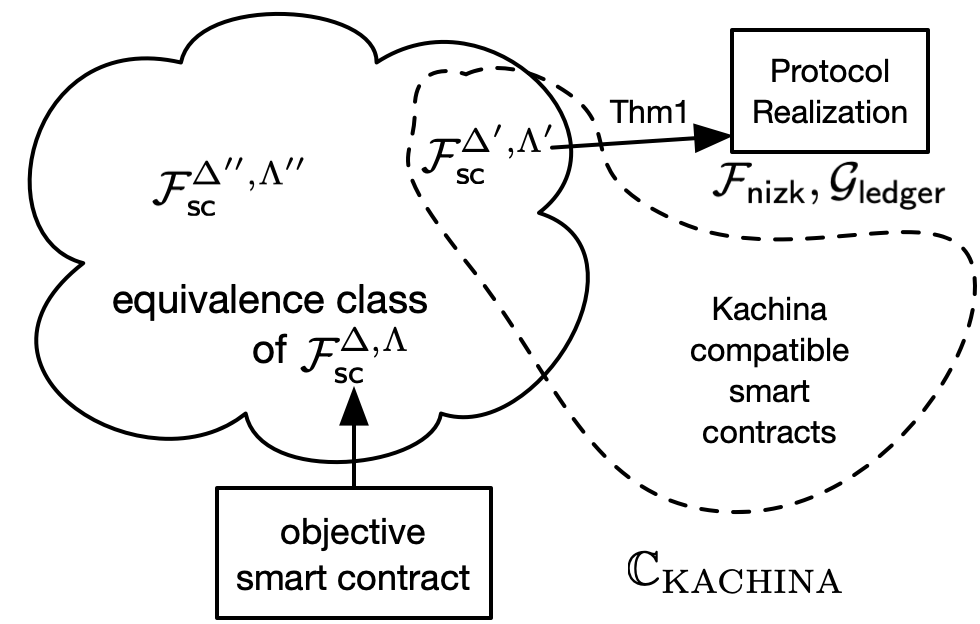
\includegraphics[scale=0.9]{the-kachina-method.png}
  \caption{An overview of the \kachina\ method to develop private smart
    contracts: 1) An intuitive description of the objective smart contract is
    developed in the form of $\fsc$. 2) A \kachina\ compatible $\fsc[\tnsfn',
    \lkgfn']$, from the set of all equivalent contracts $\fsc[\tnsfn'',
    \lkgfn'']$ is selected, and the equivalence proven. 3)
    \autoref{thm:kachina} is applied to obtain its realization.}
  \label{fig:kachinamethod}
\end{figure}

%%% Local Variables:
%%% mode: latex
%%% TeX-master: "../main"
%%% End:
